% Created 2020-11-28 sáb 19:22
% Intended LaTeX compiler: pdflatex
\documentclass[11pt]{article}
\usepackage[utf8]{inputenc}
\usepackage[T1]{fontenc}
\usepackage{graphicx}
\usepackage{grffile}
\usepackage{longtable}
\usepackage{wrapfig}
\usepackage{rotating}
\usepackage[normalem]{ulem}
\usepackage{amsmath}
\usepackage{textcomp}
\usepackage{amssymb}
\usepackage{capt-of}
\usepackage{hyperref}
\hypersetup{colorlinks=true,urlcolor=blue}
\usepackage{fancyhdr}
\fancyhead{} % clear all header fields
\pagestyle{fancy}
\fancyhead[R]{2-SMX: SOX}
\fancyhead[L]{Infraestructura]}
\usepackage{wallpaper}
\ULCornerWallPaper{0.9}{../rsrc/logos/header_europa.png}
\CenterWallPaper{0.7}{../rsrc/logos/watermark_1.png}
\author{Angel Berlanas Vicente}
\date{\today}
\title{Unidad 01 - Introducción y Virtualización}
\hypersetup{
 pdfauthor={Angel Berlanas Vicente},
 pdftitle={Unidad 01 - Introducción y Virtualización},
 pdfkeywords={},
 pdfsubject={},
 pdfcreator={Emacs 26.3 (Org mode 9.1.9)}, 
 pdflang={English}}
\begin{document}

\maketitle
\tableofcontents

\newpage
\section{Infraestructura Inicial}
\label{sec:org4429db6}

Vamos a comenzar repasando los conceptos que vimos a lo largo del año pasado de configuración
e instalación de máquinas virtuales.

Para la realización de las prácticas de este módulo, y del módulo de SER (\emph{Servicios en Red}),
utilizaremos 4 Máquinas Virtuales (cómo \emph{mínimo}).

\begin{itemize}
\item Windows 10 - \textbf{Client}
\item Windows 2019 - \textbf{Server}
\item Xubuntu 20.04 - \textbf{Client}
\item Ubuntu Server 20.04 - \textbf{Server}
\end{itemize}

A lo largo del curso estas máquinas irán comunicándose entre ellas, y las configuraremos en redes
diferentes, en estructuras diferentes, etc.

\subsection{Usuarios Administradores}
\label{sec:orgc03cd03}



Adjunto tabla resumen de las caracterísiticas de las máquinas.

\begin{longtable}{|r|c|c|c|c|}
Máquina & eths & Disco Duro & Usuario Admin & Password\\
\hline
\endfirsthead
\multicolumn{5}{l}{Continued from previous page} \\
\hline

Máquina & eths & Disco Duro & Usuario Admin & Password \\

\hline
\endhead
\hline\multicolumn{5}{r}{Continued on next page} \\
\endfoot
\endlastfoot
\hline
Win10-Client & 1 & 50GB & winadmin & Win4dmin\\
Windows-Server & 2 & 50GB & winadmin & Win4dmin\\
Xubuntu-Client & 1 & 10GB & linadmin & Lin4dmin\\
Ubuntu-Server & 2 & 15GB & linadmin & Lin4dmin\\
\end{longtable}


Todas las máquinas configurar con el parámetro de : \texttt{Usar Caché de E/S del Anfitrión}.

Por ahora, poner todas las máquinas con las tarjetas de red en \textbf{Adaptador Puente}, de tal 
manera que puedan ser accedidas desde cualquier ordenador de la red.

\subsection{Sobre la Instalación de Windows 10}
\label{sec:org8fd64de}

Para la correcta configuración y puesta en marcha de Windows luego más adelante, 
debéis utilizar la versión \textbf{Pro}, ya que será la que nos permitirá realizar las
funciones de \emph{Unión al dominio}, \emph{creación de usuarios}, etc.

\subsection{Sobre la Instalación de Ubuntu Server}
\label{sec:org7ef557a}

Debido a que los Sistemas Operativos de Servidores suelen no tener disponible
un acceso gráfico, a lo largo del curso vamos realizar todas las configuraciones
sobre \textbf{Ubuntu Server} mediante la línea de comandos.

Tareas como la ejecución de comandos, copiar y pegar desde internet, etc. Lo resolveremos
mediante \texttt{SSH} u otras herramientas parecidas.

Si para \emph{estar más cómodos} realizamos este tipo de acciones, no estamos siendo 
especialmente \emph{profesionales}.


\newpage


\begin{center}
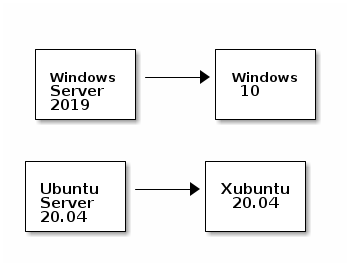
\includegraphics[width=.9\linewidth]{infraetructura.png}
\end{center}
\end{document}
